%  template.tex for Biometrics papers
%
%  This file provides a template for Biometrics authors.  Use this
%  template as the starting point for creating your manuscript document.
%  See the file biomsample.tex for an example of a full-blown manuscript.

%  ALWAYS USE THE referee OPTION WITH PAPERS SUBMITTED TO BIOMETRICS!!!
%  You can see what your paper would look like typeset by removing
%  the referee option.  Because the typeset version will be in two
%  columns, however, some of your equations may be too long. DO NOT
%  use the \longequation option discussed in the user guide!!!  This option
%  is reserved ONLY for equations that are impossible to split across 
%  multiple lines; e.g., a very wide matrix.  Instead, type your equations 
%  so that they stay in one column and are split across several lines, 
%  as are almost all equations in the journal.  Use a recent version of the
%  journal as a guide. 
%  
%\documentclass[useAMS,referee, usegraphicx]{biom}
\documentclass[useAMS, referee]{biom}
%\documentclass[useAMS, usegraphicx]{biom}
%
%  If your system does not have the AMS fonts version 2.0 installed, then
%  remove the useAMS option.
%
%  useAMS allows you to obtain upright Greek characters.
%  e.g. \umu, \upi etc.  See the section on "Upright Greek characters" in
%  this guide for further information.
%
%  If you are using AMS 2.0 fonts, bold math letters/symbols are available
%  at a larger range of sizes for NFSS release 1 and 2 (using \boldmath or
%  preferably \bmath).
% 
%  Other options are described in the user guide. Here are a few:
% 
%  -  If you use Patrick Daly's natbib  to cross-reference your 
%     bibliography entries, use the usenatbib option
%
%  -  If you use \includegraphics (graphicx package) for importing graphics
%     into your figures, use the usegraphicx option
% 
%  If you wish to typeset the paper in Times font (if you do not have the
%  PostScript Type 1 Computer Modern fonts you will need to do this to get
%  smoother fonts in a PDF file) then uncomment the next line
%  \usepackage{Times}
\usepackage{amsmath}
\usepackage[pdftex]{graphicx}
\usepackage{url}
\usepackage{bm}
\usepackage{amssymb}
\usepackage{psfrag}


%%%%% PLACE YOUR OWN MACROS HERE %%%%%

\def\bSig\mathbf{\Sigma}
\newcommand{\VS}{V\&S}
\newcommand{\tr}{\mbox{tr}}

%  The rotating package allows you to have tables displayed in landscape
%  mode.  The rotating package is NOT included in this distribution, but
%  can be obtained from the CTAN archive.  USE OF LANDSCAPE TABLES IS
%  STRONGLY DISCOURAGED -- create landscape tables only as a last resort if
%  you see no other way to display the information.  If you do do this,
%  then you need the following command.

%\usepackage[figuresright]{rotating}

%%%%%%%%%%%%%%%%%%%%%%%%%%%%%%%%%%%%%%%%%%%%%%%%%%%%%%%%%%%%%%%%%%%%%

%  Here, place your title and author information.  Note that in 
%  use of the \author command, you create your own footnotes.  Follow
%  the examples below in creating your author and affiliation information.
%  Also consult a recent issue of the journal for examples of formatting.

\title[Finite area smoothing with generalized distance splines]{Finite area smoothing with generalized distance splines}


\author{David L. Miller$^{1*}$\email{dave@ninepointeightone.net}, Simon N. Wood$^{2}$\\
$^{1}$CREEM, University of St Andrews, The Observatory, Buchanan Gardens, St Andrews KY16 9LZ, Scotland\\
$^{2}$Dept of Mathematical Sciences, University of Bath, Claverton Down, Bath BA2 7AY, U.K.
}

\begin{document}

%  This will produce the submission and review information that appears
%  right after the reference section.  Of course, it will be unknown when
%  you submit your paper, so you can either leave this out or put in 
%  sample dates (these will have no effect on the fate of your paper in the
%  review process!)

%\date{{\it Received October} 2007. {\it Revised February} 2008.  {\it Accepted March} 2008.}

%  These options will count the number of pages and provide volume
%  and date information in the upper left hand corner of the top of the 
%  first page as in published papers.  The \pagerange command will only
%  work if you place the command \label{firstpage} near the beginning
%  of the document and \label{lastpage} at the end of the document, as we
%  have done in this template.

%  Again, putting a volume number and date is for your own amusement and
%  has no bearing on what actually happens to your paper!  

%\pagerange{\pageref{firstpage}--\pageref{lastpage}} 
%\volume{65}
%\pubyear{2008}
%\artmonth{December}

%  The \doi command is where the DOI for your paper would be placed should it
%  be published.  Again, if you make one up and stick it here, it means 
%  nothing!

%\doi{10.1111/j.1541-0420.2005.00454.x}

%  This label and the label ``lastpage'' are used by the \pagerange
%  command above to give the page range for the article.  You may have 
%  to process the document twice to get this to match up with what you 
%  expect.  When using the referee option, this will not count the pages
%  with tables and figures.  

\label{firstpage}

%  put the summary for your paper here

\begin{abstract}
This version: \today %Remove this before submitting!

Spline smoothing is often used to create maps of a spatial phenomena; in this context, most smoothers use the Euclidean metric to measure the distance between data. This approach is flawed: phenomena do not conform to Euclidean geometry in their spatial distribution. Both natural and man-made barriers partition space and models should take this into account. Here we develop a finite area smoother that can be used  when the shape of the area is complex. The method is based on preserving within-area distances using multidimensional scaling. High dimensional projections of the data are necessary to avoid a loss of ordering in the points and to smooth these projections reliably Duchon splines are used. The model developed rivals the current best finite area method in prediction error terms and fits easily into larger models.
\end{abstract}

%  Please place your key words in alphabetical order, separated
%  by semicolons, with the first letter of the first word capitalized,
%  and a period at the end of the list.
%

\begin{keywords}
Generalized additive model; splines; finite area smoothing.
\end{keywords}

%  As usual, the \maketitle command creates the title and author/affiliations
%  display 

\maketitle


%  If you are using the referee option, a new page, numbered page 1, will
%  start after the summary and keywords.  The page numbers thus count the
%  number of pages of your manuscript in the preferred submission style.
%  Remember, ``Normally, regular papers exceeding 25 pages and Reader Reaction 
%  papers exceeding 12 pages in (the preferred style) will be returned to 
%  the authors without review. The page limit includes acknowledgements, 
%  references, and appendices, but not tables and figures. The page count does 
%  not include the title page and abstract. A maximum of six (6) tables or 
%  figures combined is often required.''

%  You may now place the substance of your manuscript here.  Please use
%  the \section, \subsection, etc commands as described in the user guide.
%  Please use \label and \ref commands to cross-reference sections, equations,
%  tables, figures, etc.
%
%  Please DO NOT attempt to reformat the style of equation numbering!
%  For that matter, please do not attempt to redefine anything!
\section{Introduction \label{IN}}

A typical application of spline smoothing consists of creating a a smooth of some noisy response as a function of geographical coordinates. In such cases care must be taken to account for the structure of the domain which is being modelled. If the domain is bounded (the \textit{finite area smoothing} problem) then problems can occur when the smoother does not respect the boundary shape appropriately, especially when the shape of the boundary is complex. Complexity may manifest itself as some peninsula-like feature(s) in the domain with notably different observation values on either side of the feature. Given that there is some scientific motivation as to why those parts of the domain should not affect each other, features such as peninsulae give rise to a phenomenon known as \emph{leakage}. Figure \ref{leakage} shows an example of leakage (taken from Wood, Bravington and Hedley, 2008) where the high values in the upper half of the domain leak across the gap to the lower values below and vice versa. The phenomenon is problematic since it causes the fitted surface to be mis-estimated; this can then lead to incorrect inference, which is clearly not desirable. 

% leakage example 
\begin{figure}
\centering
% trim order l b r t
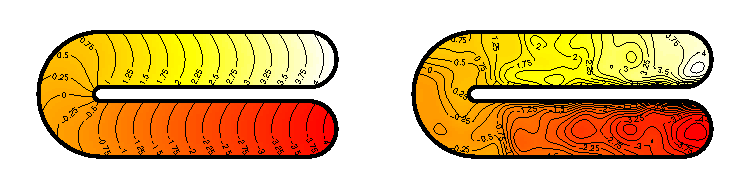
\includegraphics{figs/ramsay-leak.pdf}\\
\caption{An example of leakage on the (modified) Ramsay horseshoe (referred to simply as the Ramsay horseshoe here; Wood et al, 2008). A thin plate regression spline was fit to data sampled from the function on the top, the model smooths across the gap in the middle of the domain (bottom).}
\label{leakage}
\end{figure}

Our interests lie in harnessing such models in quantitative ecology. In such a setting the estimated function can be used to create a density map which can then be integrated over the domain to obtain an abundance estimate (e.g. Hedley and Buckland, 2004; Williams et al 2011) or as part of a larger model, taking into account nuisance spatial effects (e.g. Augustin et al 2009). 


The problem of leakage arises because of the way in which the smoother measures how near objects are to one another. Most smoothing techniques use the Euclidean metric to measure the distance between data. Clearly though, this approach is a flawed: biological populations do not conform to Euclidean geometry in their movement patterns and hence their observed positions will reflect this. Just as whales no not uniformly distribute themselves across sea and glacier, fish do not lay their eggs on land. Natural and man-made barriers carve up the landscape (and seascape), partitioning biological populations; spatial models should take this into account.

The distribution of the population may be smooth, just not necessarily over $\mathbb{R}^2$ (Wang and Ranalli, 2007). Modelling the structure of the domain correctly by embedding the extra information relating to the shape of the boundary into the model (whether this be implicitly or explicitly) allows for more accurate inference.


[[TKTKTK move this?; urggghh say something about PIRLS?! LOOK at soap paper]]Mathematically, we wish to estimate $f$ which is a smooth function of spatial coordinates giving some response, $z_i$:
\begin{equation*}
z_i = f(x_{1i}, x_{2i}).
\end{equation*}
We model $f$ as a sum of flexible (known) basis functions multiplied by coefficients (which are to be estimated). In order to avoid overfitting, penalisation of a minimisation of a sum of squares criterion is used: 
\begin{equation}
\sum_{i=1}^n \left ( z_i - \hat{f}(x_{i1},x_{i2}) \right )^2 - \lambda J\left( \hat{f} \right)
\end{equation}
where $i$ indexes the $n$ data, with $x_{i1}$ and $x_{i2}$ giving the coordinates of the data in directions 1 and 2 (e.g. the $x$-$y$ plane, longitude/latitude, etc). $\hat{f}$ is the estimated smooth function and $z_i$ is the $i^\text{th}$ response. The penalty is made up of a tunable smoothing parameter $\lambda$ and a term $J$, which is usually an integral of the squared derivatives of $\hat{f}$ (see section \ref{ss:duchon}).

An optimal degree of smoothing (i.e. an optimal $\lambda$) can then be found by optimising some prediction based criteria (GCV, etc [[TKTKTK more]]) or a (marginal) likelihood (ML, REML [[TKTKTK more here]]). The estimated smooth function $\hat{f}$ can be one part of a larger model with further (smooth) terms for other covariates (such as sea surface temperature, time of day, observer, etc). When normal errors are used, such a model is known as an additive model. Extending to the case where the response has an exponential family distribution we have the generalised additive model case (Hastie and Tibshirani, 1990; Ruppert, Wand and Carroll, 2003; Wood, 2006). An overview of recent research in the area is given in Ruppert, Wand and Carroll (2009). Often smooths of spatial coordinates are used to explain autocorrelation in the data that may confound the actual relationships of interest. Here the focus is on simple smooths of spatial location, since these are the building blocks of the more complicated models.

The cause of leakage can be characterised in two ways: either the smooth does not respect the boundary of the domain, or the smooth does not take into account the geometry of the domain (in particular with regard to the distance between points within the domain). Previous work in this area has been to combat leakage along these two lines. Work of Ramsay (2002) and Wood et al. (2008) both use a partial differential equation (PDE) boundary condition approach to try to prevent leakage, where as Wang and Ranalli (2007) and Scott-Hayward et al (????) use a graph-based distance metric to avoid smoothing across boundaries. These four main works are summarised in the next section.

Methods which consider the boundary of the domain as different from the interior are logical in situations where the edges of the domain are physically different (for example, a lake or island). However, in the case where only some boundary is land and the rest are the edges of a study region (common in cetacean studies), it does not make sense to make this distinction. For this reason we approach the problem from the perspective of using a a set of distances that are a more accurate representation of the domain.

Computing a measure of distance that is concordant with how objects in the domain would measure distance should improve predictions in finite area smoothing problems. More generally, in situations in which distances between objects are important ([[TKTKTK examples]]), being able to use an appropriate dissimilarity measure is a useful tool. Ideally we would like to fit this into the already rather large set of methods for smoothing via the GAM or mixed model framework, since they are well-developed and admit a wide set of models [[TKTKTK better]]. Since such models are firmly rooted in Euclidean space, it is necessary to project these distances into a more usual setting; the obvious candidate for performing this projection is multidimensional scaling (MDS; [[TKTKTK REF]]). There then remains only two issues. First, given that the ``quality'' of the MDS representation of the domain improves with increasing projection dimension: how many dimensions should we choose to project into? And, second, some bases fare badly in high-dimensional settings, so which basis is most suitable for smoothing in such a situation?

This article investigates the above ideas, proceeding as follows: section \ref{previous-approaches} highlights previous approaches to the problem of leakage, section \ref{proposed-model} illustrates the proposed model, section \ref{examples} gives examples of the method at work (along with comparisons to the current best methodology). Finally, section \ref{conclusion} compares the proposed method with similar approaches in the kriging literature and discusses further work.

\section{Previous approaches to the problem of leakage}
\label{previous-approaches}

As mentioned above, previous approaches run along two lines: ($i$) those that deal with the boundary directly via creating a spline basis which respects certain boundary conditions or ($ii$) using a different metric for the measurement of distances in the domain. The first two methods described below are of the former type, the third and fourth fall into this latter category.

\begin{enumerate}
\item Tim Ramsay proposed finite element $L$-splines (FELSPLINEs) in the first paper to address the finite area smoothing problem in a GAM context.

In order to find a smoother that respects the boundary, Ramsay takes a finite element approach. First triangulating the domain, then constructing a set of bivariate quadratic polynomial basis functions over each triangle, specifying that there be continuity over the edges of the triangles. By taking the FELSPLINE objective function and transforming it into a variational form (as one would for a PDE), the approximation to the minimiser of the usual GAM objective function is found (albeit with the penalty only calculated over the interior of the domain).

Since the triangulation and hence the penalty of the FELSPLINE is only calculated over the domain, and the continuity is specified over neighbouring cells, the method prevents leakage. However, although FELSPLINE does not exhibit leakage on the horseshoe given in Ramsay's paper, in practise the model makes unrealistic physical assumptions. The boundary conditions of FELSPLINE specify that the gradient is zero, along normals to the boundary. This is not always physically realistic. Wood (2008) show that by modifying the test function on horseshoe domain (as seen in Figure \ref{leakage}), the FELSPLINE performance begins to falter. FELSPLINE does not offer a realistic physical model and is therefore not a viable solution to the finite area smoothing problem in general.

\item Wood et al (2008) use a compelling physical analogy for their model: the soap film smoother. First consider the domain boundary to be made of wire, then dip this wire into a bucket of soapy water; a soap film with the same shape as the boundary will have then formed. Now consider the wire to lie in the spatial plane and the height of the soap film at a given point to be the functional value of the model. This film is then distorted smoothly by moving it vertically toward each datum locally, while minimising the surface tension in the film as a whole. 

Mathematically the soap film consists of two sets of basis functions, one that is based entirely inside the domain (a set of interior knot locations are specified) and one that is induced by the (known or estimated) boundary values. The basis functions are found by solving Poisson and Laplace's equations in two dimensions.

Although mathematically elegant, the soap film smoother is a rather complex (not to mention computationally expensive) model. The model also treats the boundary is something special, it is not clear that this is always appropriate (in particular thinking of ocean-based studies where some of the boundaries are coastlines but others are essentially arbitrary).

\item Wang and Ranalli (2007) use thin plate splines but with the usual radial distances replaced by approximate geodesic distances -- the shortest paths within the domain. To calculate the distances, a complete, weighted, undirected, graph ($G$, say) is created with a data point at each vertex and the distance between each pair of vertices as the weights on the edges. They then find the restricted graph of $G$, $G_k$, in which each vertex is only connected to its $k$ nearest neighbours. With this new, restricted, graph the geodesic distances between each pair of vertices can be calculated using Floyd's algorithm. As the authors point out, the quality of the approximation is dependent on the size of the data set and its density. At low densities the estimated geodesic distance will tend towards the Euclidean, at high densities the approximation tends, asymptotically toward the true geodesic distance (Bernstein et al, 2000). Even if  dense enough data were available, the method will be rather slow since Floyd's algorithm is cubic in the number of vertices (the size of the data set). 

\item Scott-Hayward et al. (????) improve on GLTPS by first modifying the starting graph ($G$) such that only those point pairs whose paths do not cross boundary have edges running between them and second by using a set of local radial basis functions in place of the global basis function usually used with thin plate splines (the usual global linear trends are also removed). The modification is based on selecting a rescaling of the radial distances; rather than selecting one rescaling, models with varying rescalings are averaged with weights assigned according to weighted AIC$_\text{c}$.
\end{enumerate}


All of the above methods require that knots be selected. Our method uses the eigen-decomposition method of Wood (2003) and thus avoids the knot selection problem, removing some of the subjectivity in model specification.


\section{Model definition}
\label{proposed-model}

Our model consists of a number of stages. First pairwise distances between the data must be calculated, these distances are then projected into MDS space (having selected the number of dimensions to project into) and smoothing is then performed in this new, projected space. This section describes each of these stages and discusses the technical considerations that must be taken into account. 

Here we refer to the original domain as $o$-space and the (MDS) projected domain as $p$-space. The $2$-vector $\mathbf{x}_i = (x_{1i}, x_{2i})$ is the location of the $i^\text{th}$ point in $o$-space with response $z_i$ for $i=1,\ldots,n$. 

\subsection{MDS as a transformation of space}

Multidimensional scaling (MDS) or, as it is often referred to, principle coordinates (PCO; Gower, 1966) takes distances between the observations and projects the data in such a way that Euclidean inter-point distances in the projected space are approximately the same as the distances which make up the entries of the matrix (Chatfield and Collins, 1980, Chapter 10). If the matrix of distances is of rank $n$ (if there are $n$ observations), then the projection can be in $n-1$ or fewer dimensions; a projection into 2 dimensions is a typical choice for visualisation.

Mathematically, MDS takes the ($n\times n$, symmetric) matrix of squared distances ($\mathbf{D}$, say), and eigen-decomposes it: $\mathbf{D}=\mathbf{U}\mathbf{\Lambda}\mathbf{U}^\text{T}$, where $\mathbf{U}$ is a matrix with orthogonal columns which are the eigenvectors and $\mathbf{\Lambda}$ is  a diagonal matrix of eigenvalues in decreasing absolute value order along the diagonal. Taking $\mathbf{U}\mathbf{\Lambda}^{1/2}$ and truncating it to the first $d$ columns gives a $d$-dimensional projection of the points where the distances between the points are approximately the same as the corresponding entries in $\mathbf{D}$. The $d$-vector $\mathbf{x}^*_i = (x^*_{1i}, x^*_{2i}, \ldots, x^*_{di})$ gives the corresponding locations in $p$-space, the result of a $d$-dimensional MDS projection of the within-area distances. 

If the Euclidean metric were to be used to calculate the distances between the points in $o$-space, then the resulting $p$-space would be identical up to rotation and translation to $o$-space, provided that the projection had the same number of dimensions as the original data (e.g. $o$-space and $p$-space were both 2-dimensional). Biological populations respect the intrinsic structure of their surroundings and therefore do not respect Euclidean geometry in their movement patterns in general (for example, they move around obstacles, avoid predators and track prey). When within-area distances are meaningful, it makes sense to include the structure of the domain in the model, rather than somewhat arbitrarily choosing Euclidean geometry and discarding this extra information. Since the exact particulars of how animals see the domain are distinct for each individual using a measure of within-area distance is a good proxy for how the domain is perceived for those moving within it. By within-area distance we refer to the length of the shortest path between two points within the domain where the paths do not cross the boundary. What the authors believe to be a novel algorithm for calculating such distances is given in appendix B, further discussion of the matter is given in section \ref{conclusion}.

Within-area distances calculated in $o$-space are projected into $p$-space using MDS. The within-area distances in $o$-space are approximately the same as the Euclidean distances in $p$-space. Since the GAM literature is firmly based in a Euclidean context, we can perform smoothing in $p$-space with relatively little difficulty. The approximation to Euclidean space afforded by an MDS projection of the within-area distances offers a bridge between a desire to use a well-tested (and widely used) methods, whilst also retaining information about the structure of the domain. By using within-area distances, we encapsulate information about the boundary into the model in an implicit way so that the boundary enters the model via the points rather than as a special structure (in contrast to Wood et al, 2008 and Ramsay, 2002).

In order to obtain a consistent representation of $p$-space across multiple data sets in the same domain, we first find the ``base'' MDS configuration using a sparse grid of points which cover the boundary features. This step is only used to find $p$-space reliably; the points are discarded afterward. The data locations (and any prediction locations) are inserted into this base configuration using Gower's interpolation (Gower, 1968). More detail and justification is provided in appendix A.

Preliminary experiments were carried out using a 2-dimensional projection of the distance matrix. Figure \ref{wt2-plot} shows that when a domain with peninsulae is projected using MDS with within-area distances, some of the points in the resulting configuration appear squashed. This can actually cause the ordering of the points to be lost, making the task of the smoother impossible. Further investigation showed that higher dimensional projections maintain the ordering of the points, however the number of dimensions required varied according to the shape of the domain. Before investigating how many dimensions should be used for the projection, we first look at smoothing in high-dimensional spaces.

\subsection{Smoothing with Duchon splines}
\label{ss:duchon}

Thin plate splines are a logical choice for spatial smoothing, in particular we generally want the same amount of smoothing in both directions so their isotropic property is rather useful. The formulation of Wood (2003) has the following additional desirable properties: they are eigen-based (and therefore do not require knot selection), they are relatively fast to fit and they are implemented in software (the \texttt{mgcv} package for \textsf{R}). Despite these nice properties, high-dimensional smoothing using thin plate regression splines can be rather tricky, this is because the number of unpenalised functions in the spline (the nullspace) is a function of the smoothing dimension. This leads to a model with a large nullspace, which can lead to overfitting.

When originally proposing thin plate splines in his seminal 1977 paper, Duchon actually describes a much more general set of interpolation methods; thin plate splines are just a particular example of these. This more general version of the thin plate spline (henceforth referred to as \textit{Duchon splines}) can be used for high dimensional smoothing whilst avoiding a large and complex penalty nullspace. Duchon splines have been largely neglected in statistical smoothing literature with the exception of Girosi, Jones and Poggio (1995) which discusses the connections between neural networks and GAMs. Hastie, Tibshirani and Friedman (2001, p. 168) discuss Girosi's work briefly.

A full technical exposition (from a mathematical rather than statistical point of view) is given in Duchon (1977); the aim here is only to show how the penalty works and the main differences between it and the thin plate spline penalty. 

The thin plate spline penalty (e.g. Wood, 2003) in $d$ dimensions with derivative order $m$ is :
\begin{equation}
J_{m,d} = \int \ldots \int_{\mathbb{R}^d} \sum_{\nu_1 + \dots + \nu_d=m} \frac{m!}{\nu_1! \dots \nu_d!} \left( \frac{\partial^m f \left (x_1,\dots,x_d \right )}{\partial x_1^{\nu_1} \ldots  \partial x_d^{\nu_d}} \right)^2 \text{d} x_1 \ldots  \text{d} x_d,
\label{tprs-pen}
\end{equation}
where the summation index generates all of the possible combinations of derivative orders such than their sum is still $m$ (thereby finding all the correct cross-terms for the derivatives). In order to ensure that $f$ remains continuous, $2m>d$.

It can then be shown that the minimiser of (\ref{tprs-pen}) is the thin plate spline basis:
\begin{equation}
f(\mathbf{x}) = \sum_{i=1}^n \delta_i \eta_{md}(\mathbf{x}-\mathbf{x_i}) + \sum_{j=1}^M \alpha_j \phi_j(\mathbf{x}),
\label{tprs-basis}
\end{equation}
where the first summation is a set of radial basis functions ($i$ indexing the $n$ data) and the second summation are a set of linearly independent polynomials of degree less than $m$. The terms in the second summation are unpenalized since their $m^\text{th}$ derivatives are zero. There are $M$ of these polynomials lying in the nullspace of the penalty, where $M$ is given by:
\begin{equation}
M=\begin{pmatrix} m+d-1 \\ d  \end{pmatrix}.
\label{gds-bigm}
\end{equation}
In the cases presented so far, $d$ (the MDS projection dimension) is known and $m$ is dictated by $d$, since $2m>d$. $M$ therefore increases very quickly with the number of dimensions; this is shown by the dashed line in figure \ref{nullspace-dim}. As more basis functions are included in the nullspace, the more wiggly the functions are. A large number of increasing complex, global functions which are unpenalized pose a serious threat to the fitting of parsimonious models.

\begin{figure}
\centering
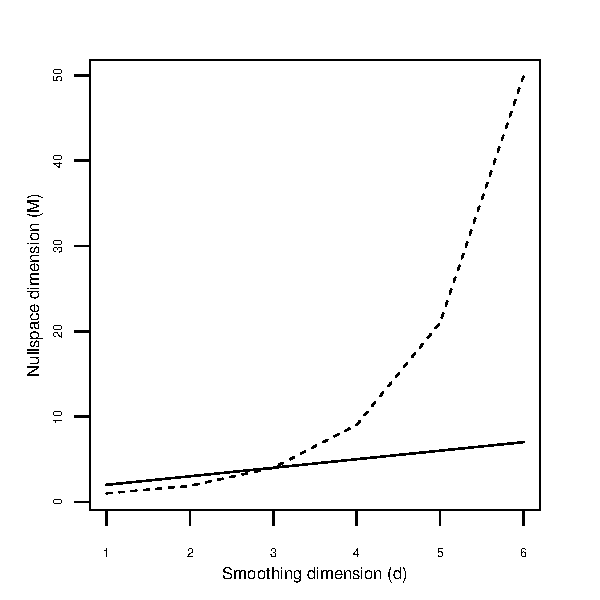
\includegraphics[width=3in]{figs/nullspace-dim.pdf} \\
\caption{Relationship between smoothing dimension ($d$) and the nullspace dimension ($M$) when $m$ (the derivative penalty order) is set to 2 for thin plate regression splines (dashed) and Duchon splines (solid). Note that as the nullspace dimension increases, the complexity of those functions in the nullspace increases too. For the thin plate splines a combination of the continuity condition that $2m>d$ and the form of $M$ (see (\ref{gds-bigm})) makes the size of the nullspace increase very quickly with smoothing dimension.}
\label{nullspace-dim}
% generated by thesis/mds/figs/nullspace-dim.R
\end{figure}

Starting from (\ref{tprs-pen}), the first step toward the more general Duchon penalty is to consider taking the Fourier transform of the derivatives before squaring and integrating them. Taking the Fourier transform of the derivatives in the penalty allows us to think of how the penalty is calculated in a different way. Rather than integrating the field of derivatives over space, the penalty is calculated from measuring the intensity of the different frequencies of the derivatives over the whole domain. Intuitively, the low frequency components of the derivatives of $f$ are likely performing a similar task to those functions in the nullspace of the penalty, where as the more complicated, high frequency components are more complicated parts of the function, likely to be the parts of $f$ that attempt to interpolate the data.

Taking the Fourier transform of the derivative terms in (\ref{tprs-pen}) yields the following penalty:
\begin{equation}
J_{m,d} = \int \ldots \int_{\mathbb{R}^d} \sum_{\nu_1 + \dots + \nu_d=m} \frac{m!}{\nu_1! \dots \nu_d!} \left ( \mathfrak{F} \frac{\partial^m f}{\partial x_1^{\nu_1} \ldots  \partial x_d^{\nu_d}} \left (  \boldsymbol{\tau}\right ) \right )^2 \text{d} \boldsymbol{\tau}.
\label{tprs-pen-ft}
\end{equation}
The penalties (\ref{tprs-pen}) and (\ref{tprs-pen-ft}) are in fact equivalent by Plancherel's theorem (e.g. Vretblad, 2003, p. 180) in the sense that they evaluate to the same numerical value.

Exploiting this frequency interpretation, it then follows to introduce a weighting into the penalty: 
\begin{equation}
\int \ldots \int_{\mathbb{R}^d} w(\boldsymbol{\tau}) \sum_{\nu_1 + \dots + \nu_d=m} \frac{m!}{\nu_1! \dots \nu_d!} \left ( \mathfrak{F} \frac{\partial^m f}{\partial x_1^{\nu_1} \ldots  \partial x_d^{\nu_d}} \left (\boldsymbol{\tau} \right ) \right )^2 \text{d} \boldsymbol{\tau}.
\label{duchon-penalty-general}
\end{equation}
The function $w$ can then be used (for example) to pick out particularly high frequencies and penalise those more than lower frequencies. Setting $w(\boldsymbol{\tau})=1, \forall \boldsymbol{\tau}$ recovers (\ref{tprs-pen}).

Duchon suggests the use of $w(\boldsymbol{\tau})= \lvert \boldsymbol{\tau} \rvert^{2s}$. This will still give a minimiser of broadly the same form as the thin plate spline functions in (\ref{tprs-basis}) but with a different $M$. First writing down this penalty:
\begin{equation}
\breve{J}_{m,d} = \int \ldots \int_{\mathbb{R}^d} \lvert \boldsymbol{\tau} \rvert^{2s} \sum_{\nu_1 + \dots + \nu_d=m} \frac{m!}{\nu_1! \dots \nu_d!}\left ( \mathfrak{F} \frac{\partial^m f}{\partial x_1^{\nu_1} \ldots  \partial x_d^{\nu_d}} \left (\boldsymbol{\tau} \right ) \right )^2 \text{d} \boldsymbol{\tau}.
\label{duchon-penalty}
\end{equation}
Again, (\ref{tprs-pen}) can be recovered from this penalty by setting $s=0$. When $s>0$ higher frequencies are penalised more than lower ones. In order to obtain smooth functions it is required that $m+s>d/2$ (this replaces the condition $2m>d$). Using a value of $s>0$ allows for high dimensional smoothing while still using lower-order penalties without yielding discontinuous functions. The less wiggly frequency components of the basis functions are penalised less. This allows some of the frequencies of  the radial basis functions to do the job of the $M$ linearly independent polynomials which were not included due to reduced nullspace size. The penalty allows the use of a reduced nullspace (in both size and complexity terms) while not sacrificing the continuity of $f$. 

One can therefore think of $s$ as a kind of ``fudge factor'' that allows the conditions on $m$ and $d$ to be relaxed. Given some fixed combination of $m$ and $d$, an $s$ can be found by simply calculating $s>d/2-m$. For the examples below, the smallest $s$ is used with $m=2$ (i.e. when second derivatives are used in the penalty), so:
\begin{equation}
s=d/2-1.
\label{duchon-s-eqn2}
\end{equation}

The solid line in Figure \ref{nullspace-dim} gives the number of functions that lie in the nullspace of penalty (\ref{duchon-penalty}), i.e. the result of using (\ref{duchon-s-eqn2}) with (\ref{gds-bigm}). For plotting $m=2$ so the derivative order is constant as the dimensionality increases, leading to a linear increase in nullspace size with the smoothing dimension.

Note that the eigen-decomposition technique for avoiding knot selection for thin plate splines from Wood (2003) can be used with Duchon splines and is used in all of the examples in this article.

\subsection{Selecting the MDS projection dimension}
\label{s:mdsdimselect}

Duchon splines allow for reliable high dimensional smoothing but how many dimensions should be used? Having a set projection dimension for every domain surely seems like a recipe for disaster, since even if this number of dimensions was set high enough to be acceptable for all domains, there would be some, simpler domains for which this would be far too high, wasting computational time and leading to non-parsimonious models. Another option would be to select the number of dimensions according to the proportion of variation in the distances explained by the projection, however this too is somewhat subjective.

Rather than using either of the above methods, the GCV score was used to final an optimal projection dimension. By fitting models with increasing projection dimension and selecting the projection with the lowest GCV score an ``optimal'' projection was found. There is no particular reason to think that the score should be unimodal in the number of dimensions, so a full search is performed. In practise an upper bound of the number of dimensions that explained 95\% of the variation in the distances was used in the analyses shown below. Figure \ref{aral-gcvplot} shows the relationship between projection dimension and GCV score for the Aral sea data analysed below.

Using GCV scores exploits the fact that the time-consuming part of the process is the calculation of the within-area distances; fitting the (G)AM is cheap in comparison (the GCV score is calculated for each model anyway, since it is used to find optimal smoothing parameters). Note that other criteria could be used; for example the ML score (the GCV score performed better in simulation, so is used here). The REML score is not suitable since the fixed effects of the model will change with the increasing projection dimension and comparison of scores is therefore not possible (Wood, 2011). 

The next section looks at some simulated examples and an analysis of data from the Aral sea. The method detailed above will be henceforth referred to as MDSDS (MultiDimensional Scaling with Duchon Splines).

\section{Examples}
\label{examples}

To illustrate the utility of the model two simulation studies are shown, followed an examples using real data. In each case MDSDS was compared with thin plate splines (which do not account for the boundary) and the soap film smoother (which does). In all cases smoothing parameters were selected by GCV. The \textsf{R} packages \texttt{mgcv} (available from CRAN), \texttt{soap} (available from \url{http://www.maths.bath.ac.uk/~sw283/simon/software.html}) and \texttt{msg} (available from \url{http://github.com/dill/msg}) were used to fit the models.

\subsection{Ramsay's horseshoe}

The horseshoe shape shown in Figure \ref{leakage} is an obvious benchmark for techniques that wish to combat leakage. Although perhaps unrealistic (and bordering on pathological), any new methods that works well on the horseshoe should have a good chance of working well in other situations. A simulation experiment was run with the same setup as in Wood et al. (2008): 200 replicates were generated at each of three error levels (standard normal noise multiplied by 0.1, 1 and 10) with sample size 600. A thin plate regression spline, (Wood, 2003), with basis size 100 and a soap film smoother with 32 interior knots  and a 40 knot cyclic  spline was used to estimate the boundary. For the MDSDS model, the basis size was set to 100 and a 20 by 20 initial grid was used for the MDS projection (see appendix A), MDS projection dimensions was selected by GCV in the range of 2 and the number of dimensions that explained 95\% of the variation in the distance matrix of the initial grid. For each realisation the mean squared error (MSE) was calculated between the true function and a prediction grid of 720 points.

\begin{figure*}
\centering
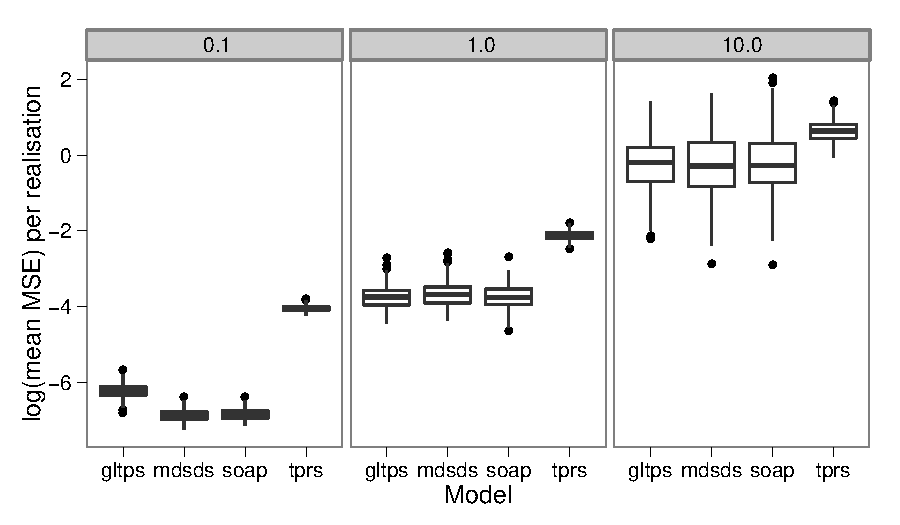
\includegraphics[width=\textwidth]{examples/ramsay/ramsay-result.pdf} \\ 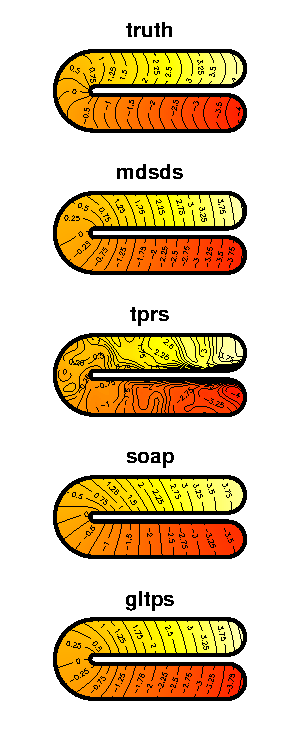
\includegraphics[width=\textwidth]{examples/ramsay/ramsay-real.pdf}
\caption{Top: boxplots of per-realisation $\log$ mean squared error at the three noise levels (rows) and sample sizes (columns). Using a paired Wilcoxon signed two-sample test, in every case the thin plate regression spline model (``tprs'') was found to be significantly worse than the soap film smoother (``soap'') at the 0.05 level. The new approach (``mdsds'') was only significantly different in two situations: sample size 300, noise level 10 (where it was worse, i.e. higher MSE) and sample size 600 with noise level 0.1 (where it was better, i.e. lower MSE). Bottom: typical predictions from the three models when the noise level was 1 and the sample size was 300. The prediciton grid used were was much finer than the one used for the MSE calculation above.}
\label{ramsay-results}
% generated by examples/ramsay/ramsay-plot.R
\end{figure*}

As can be seen in Figure \ref{ramsay-results}, the thin plate regression spline has rather poor performance in MSE terms while MDSDS performs similarly well to soap. The median number of dimensions selected for the MDS projection using GCV was 3 (max. 14, min. 2). Looking more qualitatively at the bottom part of Figure \ref{ramsay-results}, the image plots do not show any evidence of leakage.


\subsection{Peninsulae}

The results from the modified Ramsay horseshoe are encouraging. However, as mentioned above, the domain is not particularly realistic. To further explore the performance of MDSDS a more realistic domain (which attempts to mimic a coastline) was used. The domain is shown in the left panel of Figure \ref{wt2-plot}.

Again, simulations were run at a series of noise levels 0.35, 0.9 and 1.55 equating to signal-to-noise ratios of 0.50, 0.75 and 0.95. The soap film smoother used 109 internal knots and the cyclic boundary smooth used 60. The MDSDS models used an initial grid of 120 by 126 points, the basis size was 140. The thin plate regression spline basis size was also 140. Figure \ref{wt2-boxplots} shows the boxplots of the $\log$ of the MSE per realisation for each model. In the high and low noise cases, a paired Wilcoxon signed rank test showed that the soap film smoother and MDSDS were not significantly different, in the medium noise case, MDSDS was significantly better than the soap film smoother.

%tprs n= 500 noise= 0.35 -1 p= 1.447002e-34 
%mdsds n= 500 noise= 0.35 1 p= 0.2240232 
%tprs n= 500 noise= 0.9 -1 p= 2.720218e-34 
%mdsds n= 500 noise= 0.9 1 p= 3.383126e-14 
%tprs n= 500 noise= 1.55 -1 p= 5.414349e-34 
%mdsds n= 500 noise= 1.55 1 p= 0.3886599 

\begin{figure*}
\centering
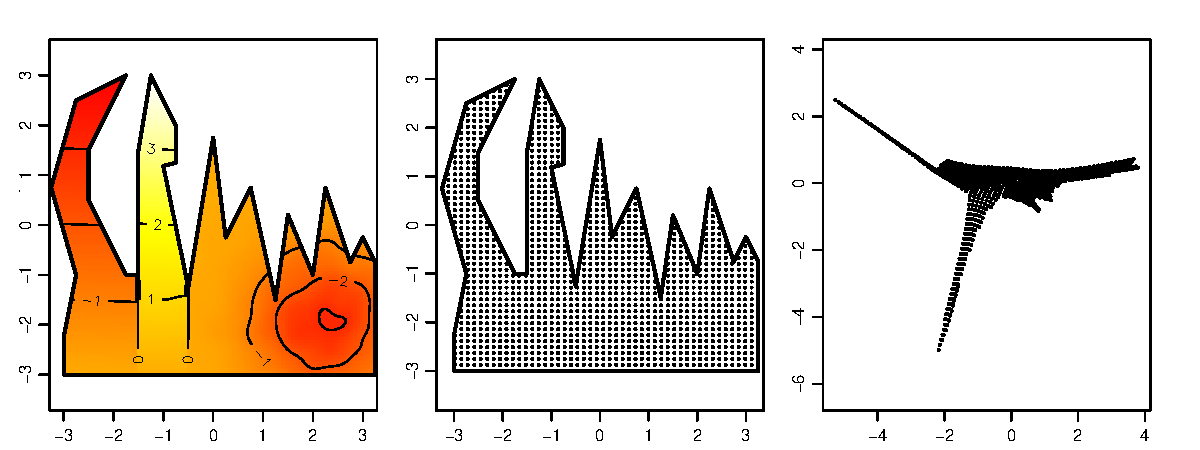
\includegraphics[width=\textwidth]{examples/wt2/wt2-plot.pdf} \\
\caption{Left to right: surface of the peninsulae domain, points in the domain and finally their projection into 2-dimensional MDS space when within-area distances are used to calculate the distance matrix. The MDS space plot shows that some squashing can happen in two dimensions. The large left peninsula and some of the smaller peninsulae have lost their ``width'' and, in fact, points within them have lost ordering.}
\label{wt2-plot}
% generated by examples/wt2/wt2-plot.R
\end{figure*}


\begin{figure*}
\centering
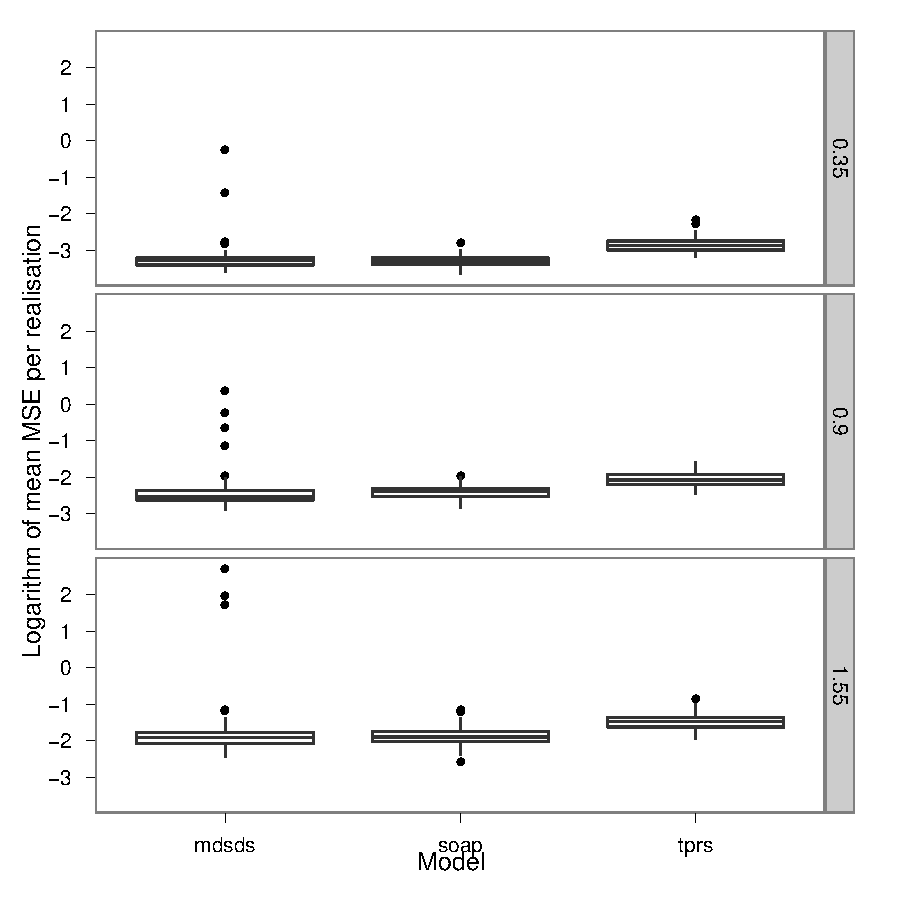
\includegraphics{examples/wt2/wt2-result.pdf} \\
\caption{Boxplots of logarithm of mean MSE per realisation for the three models tested on the peninsulae domain at three noise levels. At each noise level, the median mean MSE was lower for MDSDS than for the thin plate regression spline or soap film smoother. A paired Wilcoxon signed rank test showed that the difference between MDSDS and the soap film smoother was only significant for the 0.9 noise level (where MDSDS performed better than the soap film).}
\label{wt2-boxplots}
% generated by examples/wt2/wt2-boxplot.R
\end{figure*}



\subsection{Aral sea}

The Aral sea is located between Kazakhstan and Uzbekistan. It has been steadily shrinking since the Soviet government diverted the sea's two tributaries in order to irrigate the surrounding desert during the 1960s. The NASA SeaWifs satellite collected data on chlorophyll levels in the Aral sea over a series of 8 day observation periods from 1998 to 2002 (Wood et al, 2008). The 496 data are averages of the $38^\text{th}$ observation period. Smooths were fitted to the spatial coordinates (Northings and Eastings; kilometres from a specified latitude and longitude) with the logarithm of chlorophyll concentration (modelled with a Gamma distribution) as the response.

The models fit to the data were: a thin plate regression spline with basis size 70, MDSDS with a basis size of 70 (a 20 by 20 initial grid was used for the MDS projection) and soap film using 49 boundary knots and 74 internal knots. Using GCV for MDS projection dimension selection lead to a 5-dimensional projection (a plot of the relationship between projection dimension and GCV score can be seen in Figure \ref{aral-gcvplot}; a clear minima at 5 dimensions can be observed).

\begin{figure}
\centering
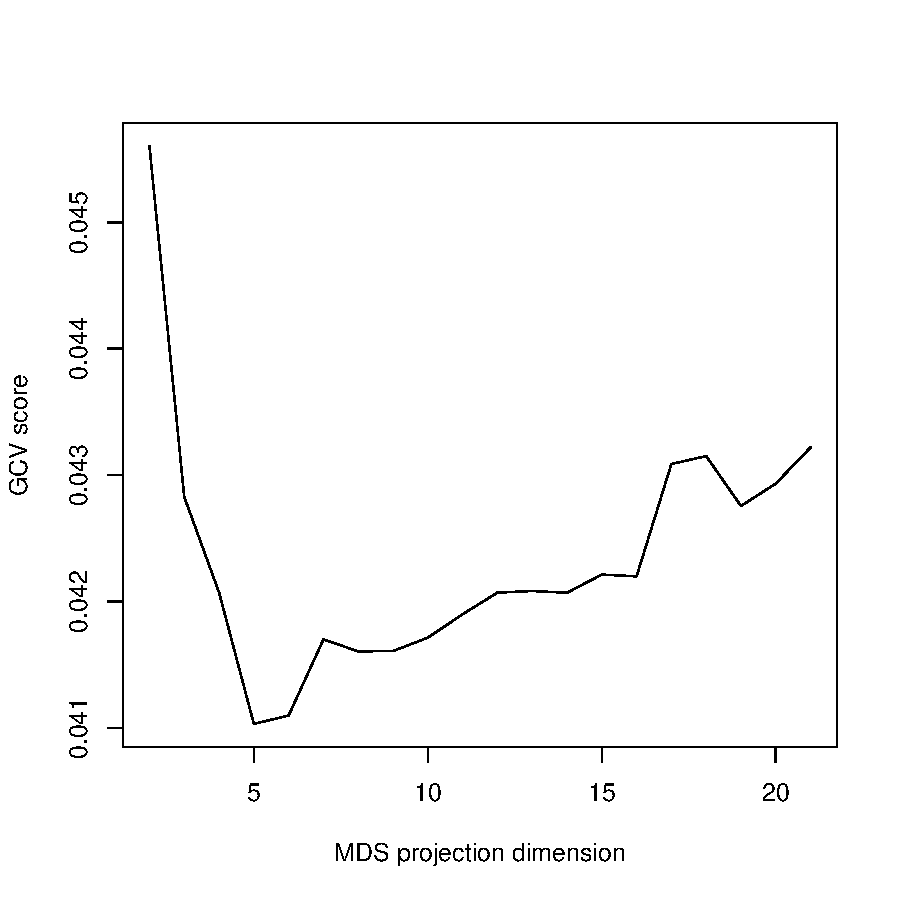
\includegraphics[width=3.5in]{examples/aral/aral-gcvplot.pdf} \\
\caption{Plot of the relationship between GCV score and MDS projection dimension for the Aral sea data set. Here a clear minima at 5 dimensions can be seen, however there is no particular reason to believe that there will always be such a pronounced optima.}
\label{aral-gcvplot}
% generated by examples/aral/aral-plot.R
\end{figure}

The models were then used to predict over a grid of 496 points to create the heat maps shown in Figure \ref{aral-plot}. The fits are broadly similar across most of the domain, with the thin plate regression spline showing some signs of leakage around (-50,-50). Both MDSDS and the soap film smoother do not have this problem. 

\begin{figure*}
\centering
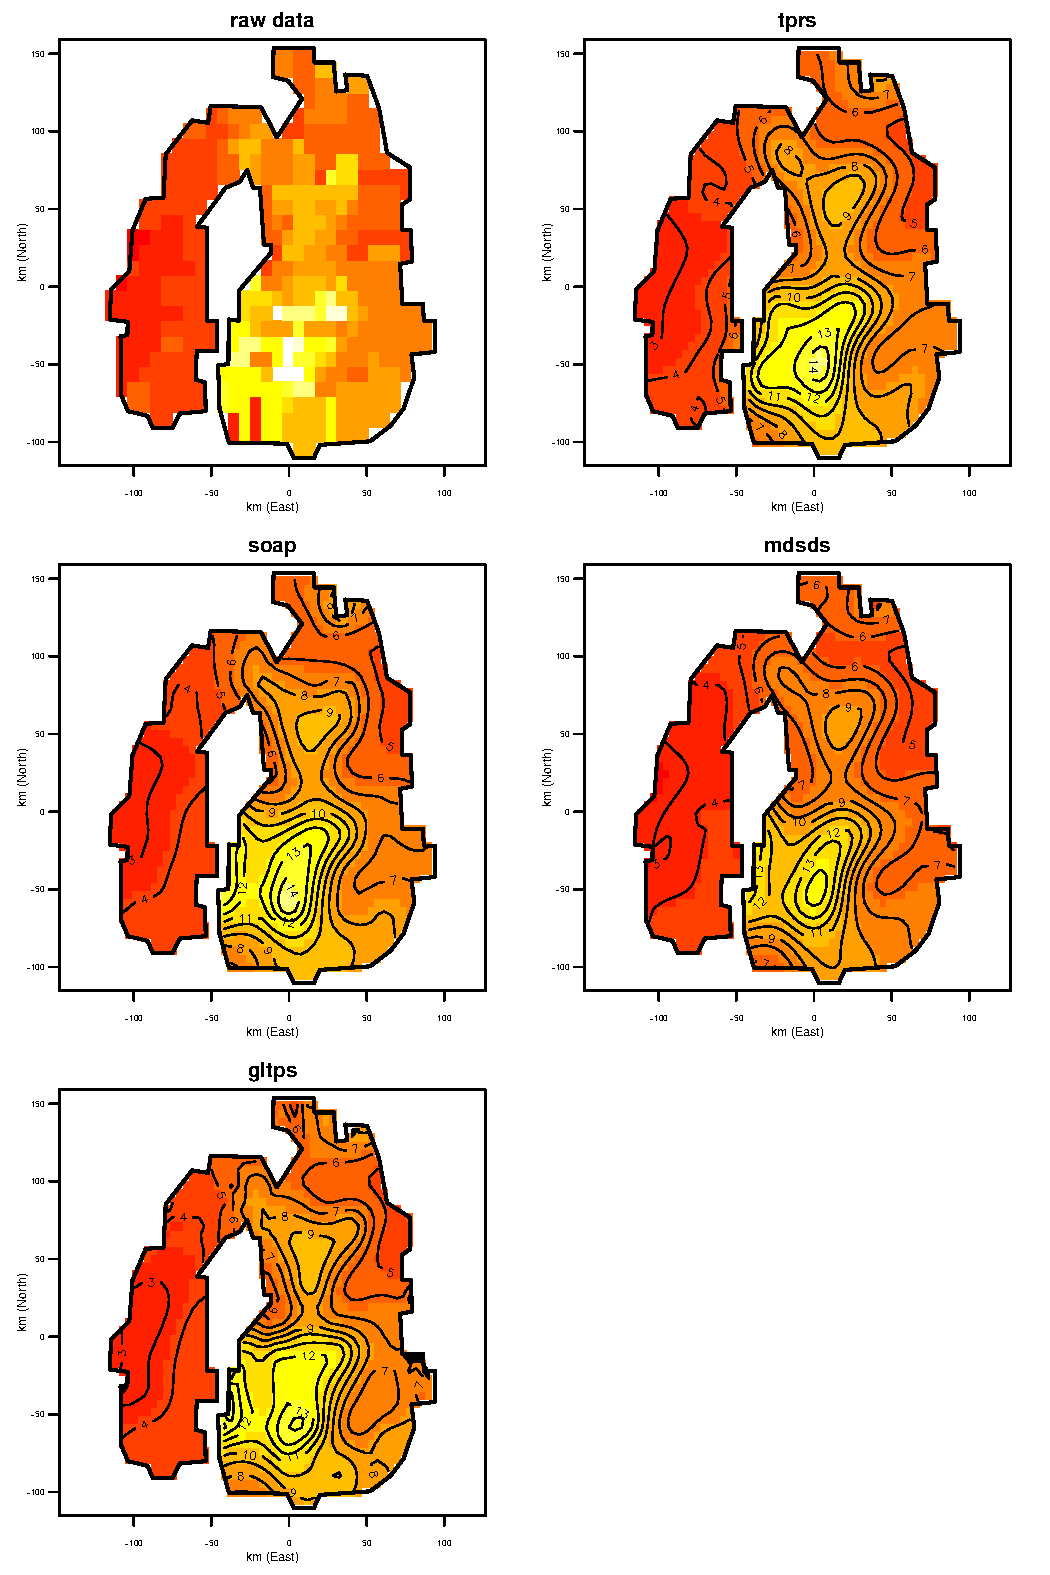
\includegraphics[width=\textwidth]{examples/aral/aral-plot.pdf} \\
\caption{Aral sea analysis. Clockwise from top left: raw data, followed by predicted surfaces for thin plate regression spline, MDSDS and the soap film smoother. The latter two avoid the leakage seen in (-50,50) region of the tin plate regression spline fit.}
\label{aral-plot}
% generated by examples/aral/aral-plot.R
\end{figure*}




\section{Discussion}
\label{conclusion}

This final section compares the MDSDS approach with similar models that have been proposed in the kriging literature. It then moves on to a discussion of further work before summing up.

\subsection{Comparison to kriging approaches}

Although the use of MDS transformations to aid smoothing using additive and generalised additive models as presented here is new, the approach has been addressed in the kriging literature previously. This section reviews the contributions made so far and compares them to the work in this article.

Kriging  (see Venables and Ripley, 2002, pp. 425--430 for a concise introduction; Schabenberger and Gotway, 2005 or Diggle and Ribiero, 2007 for a thorough treatment) consists of modelling the spatial correlation between points via the semivariogram and a spatial trend via a mean function (similar to the linear predictor in the smoothing case, although there are flavours of kriging where the mean is considered constant and/or known). Semivariogram models assume that the correlation between points is related to the distance between the points but not their position (this is known as stationarity, and comes in varying degrees, Schabenberger and Gotway, 2005, pp. 42-44). Although not specifically designed to deal with leakage issues (although leakage manifests itself as a breakdown of stationarity in a kriging context), several authors have suggested the use of some kind of transformation of the data points in space in order to maintain stationarity by approximating within-area distances with equivalent Euclidean distances via multidimensional scaling.

Kriging is focused on the explicit modelling of the correlations between points in space as a function of the distance between them via the estimation of the semivariogram. It is therefore logical that in, say, a river system the distances between points are calculated along the river's course rather than the Euclidean distance. 

For the semivariogram to be a valid covariance function, it must be positive definite or conditionally negative definite (Diggle and Ribiero, 2007, p. 47). However when non-Euclidean distances are used the semivariogram may no-longer fulfil either of these conditions (Curriero, 2006). The work of L{\o}land and H{\o}st (2003) attempts to solve this problem by using multidimensional scaling to project water distances into Euclidean space. Distances are not found exactly, a series of approximations are used rather than directly calculating the distances between the data. First the domain in question is triangulated, then the ``river distance'' between all of the nodes in the triangulation are calculated via Dijkstra's algorithm. The river distances are then projected using MDS. Finally, the data locations are mapped into the MDS space by interpolating between the grid points from the triangulation in MDS space.  The Euclidean distances in MDS space are then	 used in the estimation of the semivariogram. There are a number of issues with this approach. The authors only consider ordinary kriging (where the mean process is treated as constant). In this case spatial variation only enters the model through the semivariogram. The effect of using the MDS projected points for a spatially varying mean process (in addition to the estimation of the semivariogram) has not been investigated. Prevailing opinion is that only polynomial trends should be used for the mean process (Diggle and Ribiero, 2007, p. 57), how such an approach would perform in higher dimensions is not clear. Although the approximations used undoubtedly decrease the computational time, the validity of the approximations is not tested, especially on the fitting of the semivariogram (Jensen, Christman, and Miller, 2006). The discretisation of the domain necessary to compute the graph distance via Dijsktra's algorithm has similar pitfalls to Wang and Ranalli (2007). Jensen et al (2006) suggest using the proportion of variation explained or the Bayesian criterion of Oh and Raftery (2001) as possible metrics to perform projection dimension selection but do not fully address the issue, resorting to 2-dimensional projections. Neither of the proposed selection methods take into account the effect that the dimension of the MDS projection has on the overall model (as discussed in section \ref{s:mdsdimselect}). Boisvert, Manchuk and Deutsch (2009) suggest that to best approximate the distances, an $n-1$ dimensional projection of the distance matrix (if there are $n$ data, or triangulation nodes) be used. Such a projection does, of course, provide the best approximation however, they go on to point out that the use of such a high-dimensional projection could lead to numerical problems. Interpolating to find the distances in higher dimensions may also have it's own issues and so the approximations may run into further problems. In all of these works the MDS projection is being used to approximate the within-area distances by a set of distances obeying the rules of a Euclidean metric which is the criterion given by Curriero (2006) to ensure the semivariogram is valid. Unlike in the material presented here, the MDS point configuration itself is not being used except to obtain a Euclidean approximation to the distances matrix so that the semivariogram can be estimated.

In general kriging methods suffer from having developed as an \textit{ad hoc} set of tools used in the mining industry (Diggle and Ribiero, 2007, preface). Although much work has been done to improve the mathematical basis of kriging, models are not as flexible as GAMs, in particular the incorporation of other covariates, temporal effects and random effects is not straight forward as it is for additive and generalized additive models (in both theory and practise).

\subsection{Further work}
\label{s:furtherwork}

As it stands distance generation is seen as a black box procedure to the model. This means that any procedure that can generate a distance matrix can be used. Instead of using the algorithm given in appendix B, an algorithm that uses a discretisation of space could be used (for example the A$^*$ algorithm; Hart, Nilsson and Raphael, 1968). The examples presented here only consider smoothing inside of simple polygons since the within-area distance algorithm given in appendix B can only find shortest paths inside such shapes. This excludes domains with islands in them, which can occur in ship-board studies. This could be worked-around using other shortest path algorithms. In such cases the MDS projection may not adequately prevent leakage. For example, imagine taking the MDS projection of an annulus, having used within-area distances. This would lead to an expanded annulus since the annulus itself is symmetric, the shape would be the same, just the distance between points (across the hole) would reflect their distance around the ring. Once this is extended to the multi-ring case, it is not clear whether this would still prevent leakage.

It might also be interesting to investigate the use of other measures to populate the distance matrix. Moving into three dimensions could be useful, finding the shortest path over say a mountain range, which would include minimising changes in altitude as well as avoiding obstacles. Alternatively, a cost based distance approach that takes into account fuel cost or taking into account difficult conditions (e.g. a bog or ford that can be crossed but at additional cost in terms of effort or time). One issue with such general cost-distance approach might be that the ``distance'' measure could turn out to be non-metric. That is, that the distance from A to B is not the same as the distance from B to A (for example going against versus going with the flow of a river). In this case non-metric MDS must be used, this relies only on the rankings of the data and discards other information, which is probably undesirable.


\subsection{Final comments}

This article has investigated a problem which arises when smoothing in a finite area when the boundary is a complex shape: leakage. We proposed a new solution to this problem for the additive and generalized additive model framework using a combination of multidimensional scaling, within-area distances and the Duchon spline basis. In comparison with the current ``best' approach (soap film smoothing) MDSDS was found to be competitive in MSE terms.

Initial investigations looked the the utility of the Schwarz-Christoffel transformation (Driscoll and Trefethen, 2002) as suggested by Paul Eilers (in a seminar at University of Munich in 2006). However it was soon found that such a conformal mapping (from some arbitrary polygon defining the boundary of the domain to, say, a rectangle) was far to prescriptive and did not allow for the flexibility necessary for a domain transformation approach. The Schwarz-Christoffel transform failed to preserve the distances between objects, causing artefacts to appear that were significantly more problematic than the leakage which it sought to prevent. Using MDS preserves the between-point distances, since these are encoded in the distance matrix. The discovery that 2-dimensional projections produced by MDS can cause the ordering of the points to be lost explained the poor performance of the model up to that point. These problems were overcome by projecting into higher dimensions and using Duchon splines to perform reliable high dimensional smoothing.


\section*{Acknowledgements}

David wishes to thank EPSRC for financial support during his PhD.


% Appendices
\section*{Appendix A - Using starting grids for stable MDS projection}

In many applications of multidimensional scaling, points are simply projected and no further points are added to the resulting configuration. However in the situations discussed here, there are at least two phases in the procedure. First the data which have been collected are projected and second prediction points must also be projected. Assuming that these sets of points are not identical, it is essential for the two to have the same coordinate systems for reliable inference to be performed. 

Gower (1968) proposes a method for inserting new points into an existing MDS configuration. Gower shows that performing MDS on a dataset is equivalent to performing MDS on a reduced set of points and then inserting the remaining points. However in the within-area distance case there can the potential problems if the reduced set of points does not encapsulate enough information about the domain. The only place that the boundary enters the model is through the MDS configuration and in turn, the MDS configuration's only influence from the boundary is via the distances in $\mathbf{D}$. In a spatial setting one can imagine the case in which samples were not taken from one part of the domain of interest (for example, there may be no observations in a particular peninsulae) and in that case the resulting MDS configuration would differ from a configuration when data that was evenly sampled over the whole domain was used. Ensuring that different analyses on the same domain of interest yield consistent results is essential.

When Euclidean distances are used to calculate $\mathbf{D}$, the criterion needed so that the resulting space is the same (in the sense given above, that insertion into a reduced point set is the same as mapping the complete point set) is that there is one more point used to create the MDS configuration than there are dimensions in the space in which they reside (provided the points are not collinear; de Silva and Tenenbaum, 2004). There is no similar criteria for within-area distances and it is unclear what form such a criterion would take.

This problem can be rectified by using an appropriately spaced grid over the domain to calculate the eigen-decomposition, thus ensuring that the whole domain is covered. Provided that the grid is fine enough to catch all of the important features in the boundary of the domain, the problems above should not arise.

\section*{Appendix B - Algorithm for the calculation of within-area distances}

It is assumed above that the matrix of distances, $D$, is known; this appendix describes (what the authors believe to be) novel algorithm to find shortest paths within a given domain. Note that paths between point pairs in \textit{simple} polygons (i.e. those polygons without holes) are considered. Although this limits the types of domains that can be addressed, it does make the shortest path algorithm simpler, since the shortest path is unique. Whether MDS projections in such situations would be useful is another matter (see section \ref{s:furtherwork}).

Both of the algorithms for finding within-area distances discussed above (the graph-based methods used by Wang and Ranalli (2007) and Scott-Hayward et al (????) and the $\text{A}^*$ algorithm of Hart et al (1968)) rely on the discretisation of the domain of interest. This discretisation of the domain is undesirable since the results then become dependent on the resolution of the discretisation of the domain, even if a high enough resolution can be used the computational cost becomes prohibitively expensive for such methods. It would be preferable to have an elementary algorithm (i.e. one not relying on complex data structures or extensive theory) for finding the shortest path within the polygon.

The algorithm is defined as follows, it will be helpful to look at the example in Figure \ref{wdia} while reading.

Let the domain boundary be some polygon, $\Gamma$. Given that there is no direct path within the domain between two points ($p_1$ and $p_2$, say), the algorithm proceeds as follows to create a path, $\mathcal{P}$, which is an ordered set of vertices:
\begin{enumerate}
\item (INIT) Start by drawing a line between $p_1$ and $p_2$ (Figure \ref{wdia}, ($i$)). Start the path as the lines from $p_1$, $p_2$ to their nearest intersection with the boundary of $\Gamma$ ($p_1^1$, $p_2^1$, say). Then form two paths. The first path from $p_1^1$ to $p_2^1$ ($\mathcal{P}_1$) contains the vertices of $\Gamma$ found moving along the boundary from $p_1^1$ to $p_2^1$. The second ($\mathcal{P}_2$), is found by taking the path from $p_1^1$ to $p_2^1$ in the other direction around the boundary, ie. the vertices of $\Gamma$ not in the first path. It is easy to see that $\{\mathcal{P}_1 \cup \mathcal{P}_2\} \setminus \{p_1^1, p_2^1\} = \Gamma$. The DELETE step (below) is then performed on $\mathcal{P}_1$ and $\mathcal{P}_2$, removing any superfluous vertices. Finding the length of $\mathcal{P}_1$ and $\mathcal{P}_2$ and choosing the shorter ($\mathcal{P^*}$), the initial path is formed as $\mathcal{P}=(p_1,p_1^1,\mathcal{P}^*,p_2^1,p_2)$. 

In Figure \ref{wdia}, ($iii$), $\mathcal{P}_1$ is marked in green and is chosen to form the initial path, $\mathcal{P}=(p_1,p_1^1,\mathcal{P}_1,p_2^1,p_2)$, as $\mathcal{P}_1$ is shorter than $\mathcal{P}_2$, in red.

\item (DELETE) Given a triple of vertices, $(v_i, v_{i+1}, v_{i+2}) \in \mathcal{P}$ , if the line between $v_i$ and $v_{i+2}$ is shorter than the path $(v_i, v_{i+1}, v_{i+2})$ and the line between $v_i$ and $v_{i+2}$ lies inside $\Gamma$ then delete $v_{i+1}$ (Figure \ref{wdia}, ($iv$) and ($vi$)). The entire path is iterated over ($i=1,\ldots,N-2$, if there are $N$ vertices in $\mathcal{P}$)  deleting all superfluous vertices until there are no changes in successive runs. 

For example in Figure \ref{wdia} ($iii$), $v_2$ is deleted from $\mathcal{P}$ because the path straight between $v_1$ and $v_3$ is shorter, and within $\Gamma$.

\item (ALTER) Given a triple of vertices $(v_i, v_{i+1}, v_{i+2}) \in \mathcal{P}$, if the candidate replacement path $\mathcal{P}_{ID}$ is shorter than the path $(v_i, v_{i+1}, v_{i+2})$ then replace $(v_i, v_{i+1}, v_{i+2})$ with $\mathcal{P}_{ID}$ (Figure \ref{wdia}, ($v$)). The candidate replacement path, $\mathcal{P}_{ID}$, is calculated by running INIT with $p_1$ and $p_2$ replaced by $v_i$ and $v_{i+2}$.

For example in Figure \ref{wdia} ($iv$), the path $(v_1, v_2, v_3)$ is longer than the path $\mathcal{P}_{ID}=(v_1, v^1_2, v_3)$ (green dashed line in ($iv$)) so the former is replaced with the latter in $\mathcal{P}$. The path created by INIT is marked as $\mathcal{P}_{I}$ in  ($iv$) in red.

\item (ITER) Iterate further DELETE and ALTER steps (in pairs) until there has been no change in $\mathcal{P}$ from one run to the next (i.e. convergence) (Figure \ref{wdia}, ($vi$)).
\end{enumerate}

% diagram for finding the shortest path in W
\begin{figure}
% trim order l b r t
%\psfrag{exp1}[]{$\mathcal{P}_1$}
%\includegraphics[trim=0in 0.5in 0in 0.25in][figs/wdia.pdf} \\
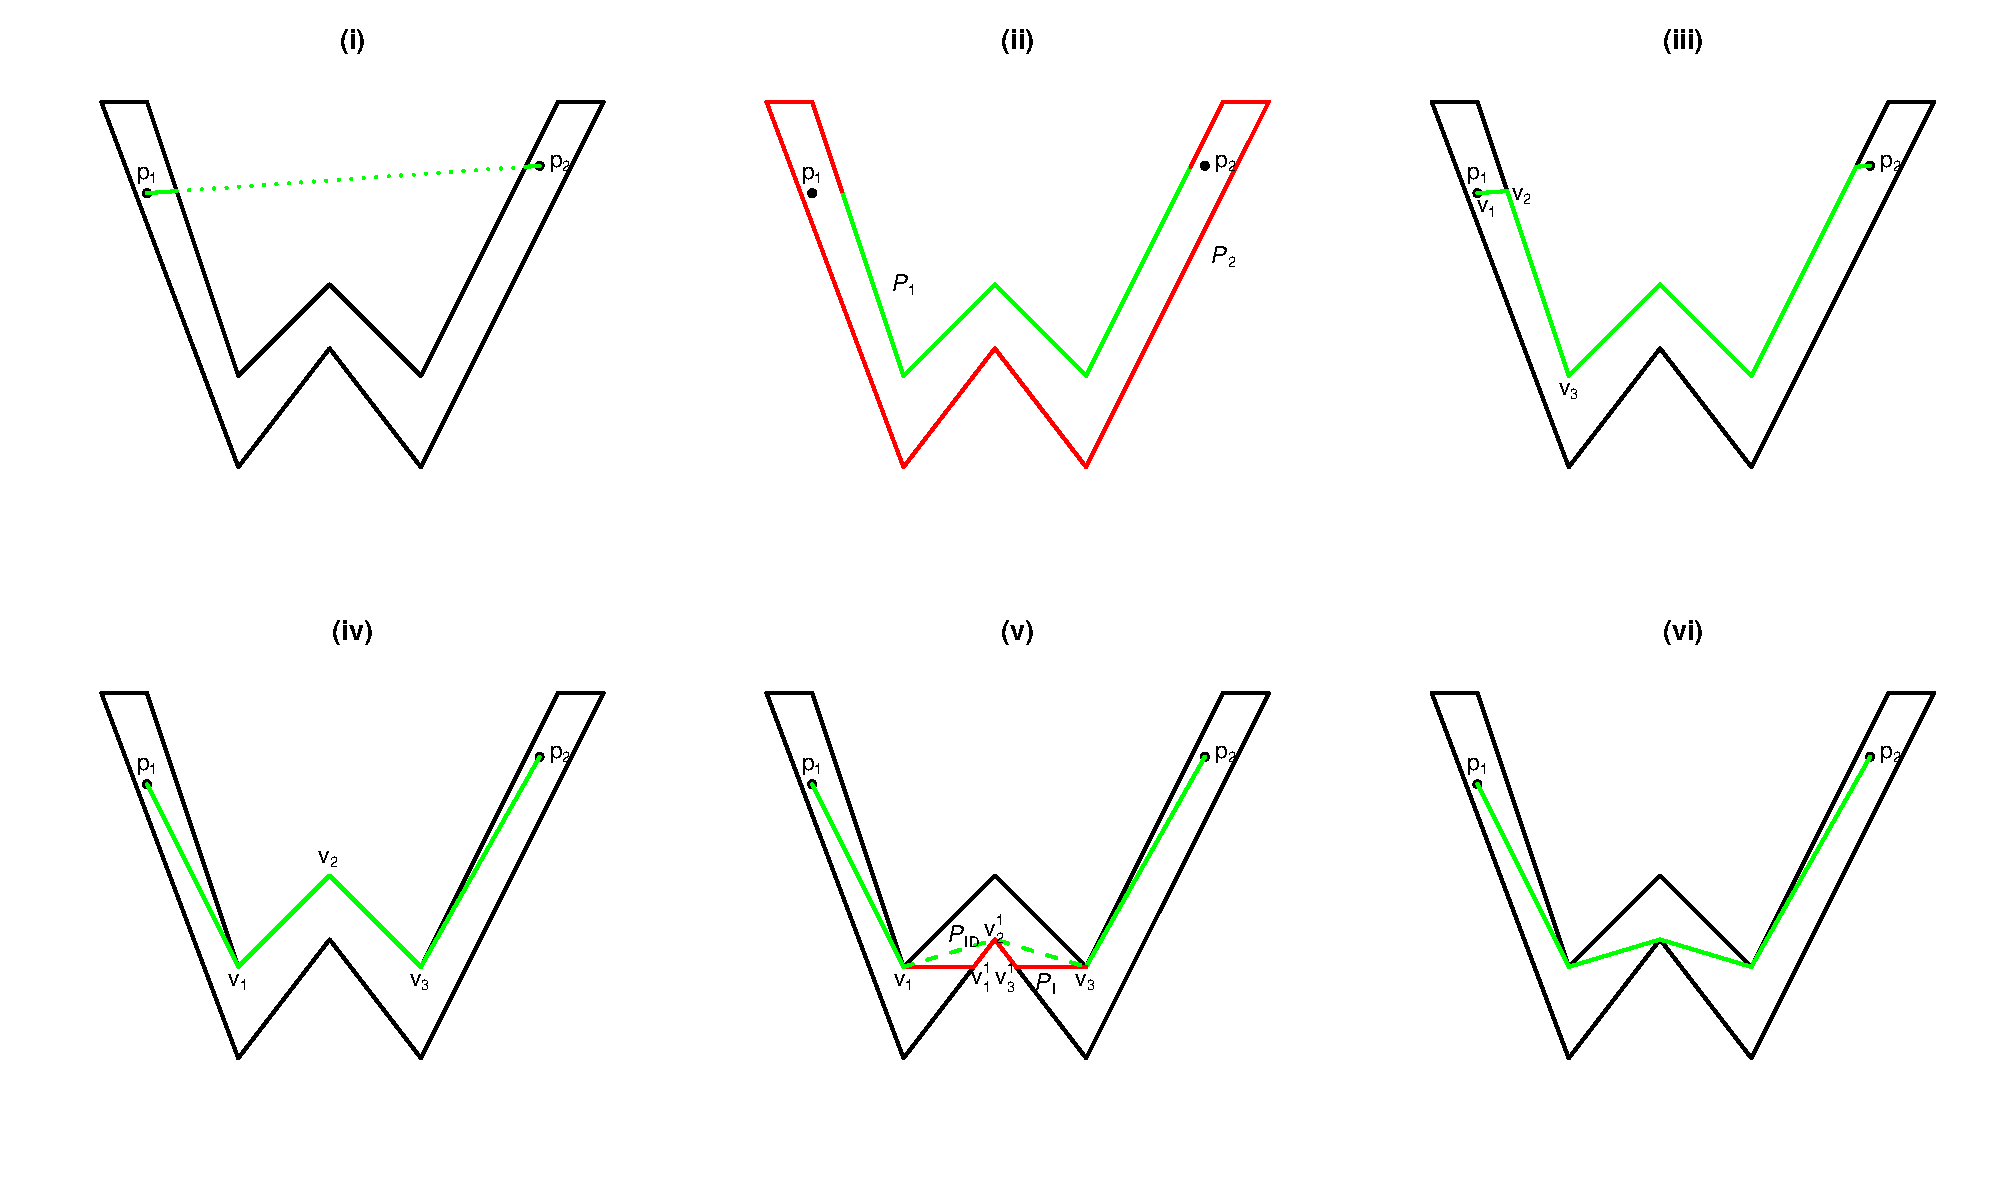
\includegraphics[angle=90, height=\textheight,trim=0in 0.5in 0in 0.25in]{figs/wdia.pdf} \\
\caption{The green lines in ($i$) to ($vi$) show the steps forming the shortest path as the algorithm progresses from initial state to final, shortest path (bottom right). See appendix B for more details.}
\label{wdia}
% generated by figs/distanceexplanation.R
\end{figure}

Of course, if there is a direct path between $p_1$ and $p_2$ then the Euclidean distance between the points can be used and the above algorithm is not run.

Although the authors were not able to prove theoretically that the algorithm will always converge to the shortest path, it is clear at least the the algorithm will always converge (since this only requires that there be no change in the path for two consecutive iterations). Extensive simulations showed that the algorithm gave sensible results.


\subsection*{Speed improvement via partial path calculation}

It is often the case that the points for which the within-area distances are required form a grid (for example, the initial MDS grid setup, or when prediction points need to be found). This grid setup can be exploited since there are many sets of paths that are rather similar. These paths may perhaps only differ in their final vertex. When this is the case much computational time is wasted calculating similar paths, it would be useful to exploit this problem and use it to increase the speed of the path calculation.

By appending the points between which the within-area distance is required to either end of one of a series of pre-calculated base paths, then optimising this new path using the DELETE and ALTER steps as before,  the computational time taken to find the paths is reduced. Using base paths removes the expensive calculation in the middle of the path, where the bulk of the interactions with the boundary take place.

The algorithm is as follows, with notation and routines (INIT, DELETE, ALTER and ITER) identical to those above:
\begin{enumerate}
 \item Begin by creating a sparse grid of within the simple polygon $\Gamma$ and calculate the ($M$, say) non-Euclidean within-area paths between all pairs of points in the grid, as above. Store these paths as $\mathcal{P}_1,\ldots, \mathcal{P}_M$.
\item For each unique pairing of $p_i$ and $p_j$ in the full data set, calculate the path using one of the following:
	\begin{enumerate}
	\item Find a $\mathcal{P}_k$ such that the path between $p_i$ and one end of $\mathcal{P}_k$ and $p_j$ and the other end of $\mathcal{P}_k$ is Euclidean within $\Gamma$. Join $p_i$ and $p_j$ onto the appropriate ends of $\mathcal{P}_k$ and alternate between DELETE and ALTER steps until convergence.
	\item If no $\mathcal{P}_k$ can be found calculate the path between $p_i$ and $p_j$ as above. 
	\end{enumerate}
\end{enumerate}

Note that those paths between points in the sparse grid which are Euclidean are not stored since it is always at least as expensive to store, add and optimise those paths then calculating them from scratch. If the required path is Euclidean anyway, then retrieving a Euclidean path, adding in $p_i$ and $p_j$, and then iterating over ALTER and DELETE steps to make it both the shortest and a Euclidean path will take longer than just creating a Euclidean path to begin with. If the path between $p_i$ and $p_j$ is non-Euclidean then the non-Euclidean part of the path must lie outside $\mathcal{P}_k$ (by definition, if $\mathcal{P}_k$ were Euclidean) and therefore will take the same number of operations to find the boundary crossing points and calculate the shortest path around the feature locally as it will to calculating the whole path from scratch.

Implementation of this algorithm (in C) reduced time to fit MDSDS to the peninsulae domain above (without MDS dimension selection) from 84 seconds to 18 seconds on a MacBook Air (2,1) with a 1.86GHz Intel Core 2 Duo processor.

This algorithm could be further improved by finding schemes for the layout of starting grids and perhaps adapting the methods described in L{\o}land and H{\o}st (2003) to approximate the distances using a triangulation, would certainly increase performance (although perhaps at the price of accuracy).

\begin{thebibliography}{99}

\bibitem{} Augustin, N.H., Musio, M., von Wilpert, K., Kublin, E., Wood, S.N. and Schumacher, M. (2009). 
Modeling spatiotemporal forest health monitoring data. \textit{Journal of the American Statistical Association} \textbf{104}(487), 899--911.

\bibitem{} Bernstein, M., de Silva, V., Langford, J.C., and Tenenbaum, J.B. (2000). Graph approximations to geodesics on embedded manifolds. Technical report.

\bibitem{} Boisvert, J.B., Manchuk,  J.G. and Deutsch, C.V. (2009). Kriging in the presence of locally varying anisotropy using non-{E}uclidean distances. \textit{Mathematical Geosciences} \textbf{41}, 585--601.

\bibitem{} Chatfield, C. and Collins, A.J. (1980). \textit{Introduction to multivariate analysis}. CRC Press.

\bibitem{} Curriero, F. (2006). On the use of non-{E}uclidean distance measures in geostatistics. \textit{Mathematical Geology} \textbf{38}(8), 907--926.

\bibitem{} Diggle, P.J. and Ribeiro, P.J. (2007). \textit{Model-based Geostatistics}. Springer.

\bibitem{} 	Driscoll, T.A. and Trefethen, L.N. (2002). \textit{Schwarz-Christoffel Mapping}. Cambridge University Press.

\bibitem{} Girosi, F., Jones, M. and Poggio, T. (1995). Regularization theory and neural networks architectures. \textit{Neural computation}, \textbf{7}, 219-269.

\bibitem{} Gower, J.C. (1966). Some distance properties of latent root and vector methods used in multivariate analysis. \textit{Biometrika}, \textbf{53}(3 and 4), 325--338.

\bibitem{} Gower, J. C. (1968). Adding a point to vector diagrams in multivariate analysis. \textit{Biometrika}, \textbf{55}(3), 582--585.

\bibitem{} Hart, P. E., Nilsson, N. J. and Raphael, B. (1968). A Formal Basis for the Heuristic Determination of Minimum Cost Paths. \textit{IEEE Transactions on Systems Science and Cybernetics SSC4} \textbf{4}(2), 100--107.

\bibitem{} Hastie, T. and Tibshirani, R. (1990). \textit{Generalized Additive Models}. Chapman \& Hall.

\bibitem{} Hastie, T., Tibshirani, R. and Friedman, J. (2001). \textit{Elements of Statistical Learning}. Springer.

\bibitem{ } Hedley, S.L. and Buckland, S.T. (2004) Spatial Models for Line Transect Sampling. \textit{Journal of Agricultural, Biological, and Environmental Statistics} \textbf{9}(2), 181--199.

\bibitem{} L{\o}land, A. and H{\o}st, G. (2003). Spatial covariance modelling in a complex coastal domain by multidimensional scaling. \textit{Environmetrics} \textbf{14}(3), 307--321.

\bibitem{} Jensen, O.P., Christman, M.C. and Miller, T.J. (2006). Landscape-based geostatistics: a case study of the distribution of blue crab in {C}hesapeake {B}ay. \textit{Environmetrics} \textbf{17}(6), 605--621.

\bibitem{} Marra, G. and Radice, R. (2010). Penalised regression splines: theory and application to medical research. \textit{Statistical Methods in Medical Research}, 19, 107--125.

\bibitem{} Miller, D.L. (2011) \textit{On smooth models for complex domains and distances}. PhD thesis, University of Bath.

\bibitem{} Oh, M-S and Raftery, A.E. (2001). Bayesian multidimensional scaling and choice of dimension. \textit{Journal of the American Statistical Association}, \textbf{96}(455), 1031--1044.

\bibitem{} Ramsay, T. (2002). Spline smoothing over difficult regions. \textit{Journal of the Royal Statistical Society: Series B} \textbf{64}(2), 307--19.

\bibitem{} Ruppert, D., Wand, M.P. and Carroll, R.J. (2003). \textit{Semiparametric Regression}. Cambridge University Press.

\bibitem{} Ruppert, D., Wand, M.P. and Carroll, R.J. (2009). Semiparametric regression during 2003--2007. \textit{Electronic Journal of Statistics}, \textbf{3}, 1193--1256.

\bibitem{} Scott-Hayward, L.A.S., Mackenzie, M.L., Donovan, C.R., Walker, C.G. and Ashe, E. (????) Complex Region Spatial Smoother (CReSS). \textit{A Journal}.

\bibitem{} Shabenberger, O. and Gotway, C.A. (2005). \textit{Statistical methods for spatial data analysis}. CRC Press.

\bibitem{} de Silva, V. and Tenenbaum, J.B. (2004). Sparse multidimensional scaling using landmark points. Tech report, Stanford University.

\bibitem{} Venables, W.N. and Ripley, B.D. (2002). \textit{Modern applied statistics with S}. Springer.

\bibitem{} Vretblad, A. (2003). \textit{Fourier Analysis and Its Applications}. Springer.

\bibitem{} Wang, H. and Ranalli, M.G. (2007). Low-rank smoothing splines on complicated domains. \textit{Biometrics} \textbf{63}(1), 209--217

\bibitem{} Williams, R., Hedley, S.L., Branch, T.A. and Bravington, M.V., Zerbini, A.N. and Findlay, K.P. (2011). Chilean Blue Whales as a Case Study to Illustrate Methods to Estimate Abundance and Evaluate Conservation Status of Rare Species. \textit{Conservation Biology} \textbf{25}(3), 526--535.

\bibitem{} Wood, S.N. (2003). Thin plate regression splines. \textit{Journal of the Royal Statistical Society: Series B}, \textbf{65}(1) 95--114.

\bibitem{} Wood, S.N. (2006). \textit{Generalized Additive Models: An Introduction with R}. Chapman \& Hall.

\bibitem{} Wood, S.N. (2011). Fast stable restricted maximum likelihood and marginal likelihood estimation of semiparametric generalized linear models. \textit{Journal of the Royal Statistical Society: Series B}, \textbf{73}(1), 3--36.

\bibitem{} Wood, S.N., Bravington, M.V. and Hedley, S.L. (2008). Soap film smoothing. \textit{Journal of the Royal Statistical Society Series B} \textbf{70}(5), 931--55.

\end{thebibliography}


\label{lastpage}

\end{document}

